\subsection{(W) Handling Head on Approach}\label{sec:handlingHeadOnApproach}
    \begin{itemize}
        \item Describe VFR manuever in details
        \item Emphatize on IFR required parameters - angle of approach range, safety margin
        \item introduce virtual roundabout idea - minimizes wake turbulence and enables thick attendants flow on virtual airline in selected flight level (this is actually one of Boeing concepts for next gen ATM).
        \item Refer to conditions and triggers from collision case resolution algorithm.
        \item I prefer structure-process flow, due to my software viewpoint bias, this section can be shifted before \ref{sec:collisionCase}
    \end{itemize}
    \begin{figure}[H]
    	\centering
        \begin{subfigure}{0.45\textwidth}
        	\centering
            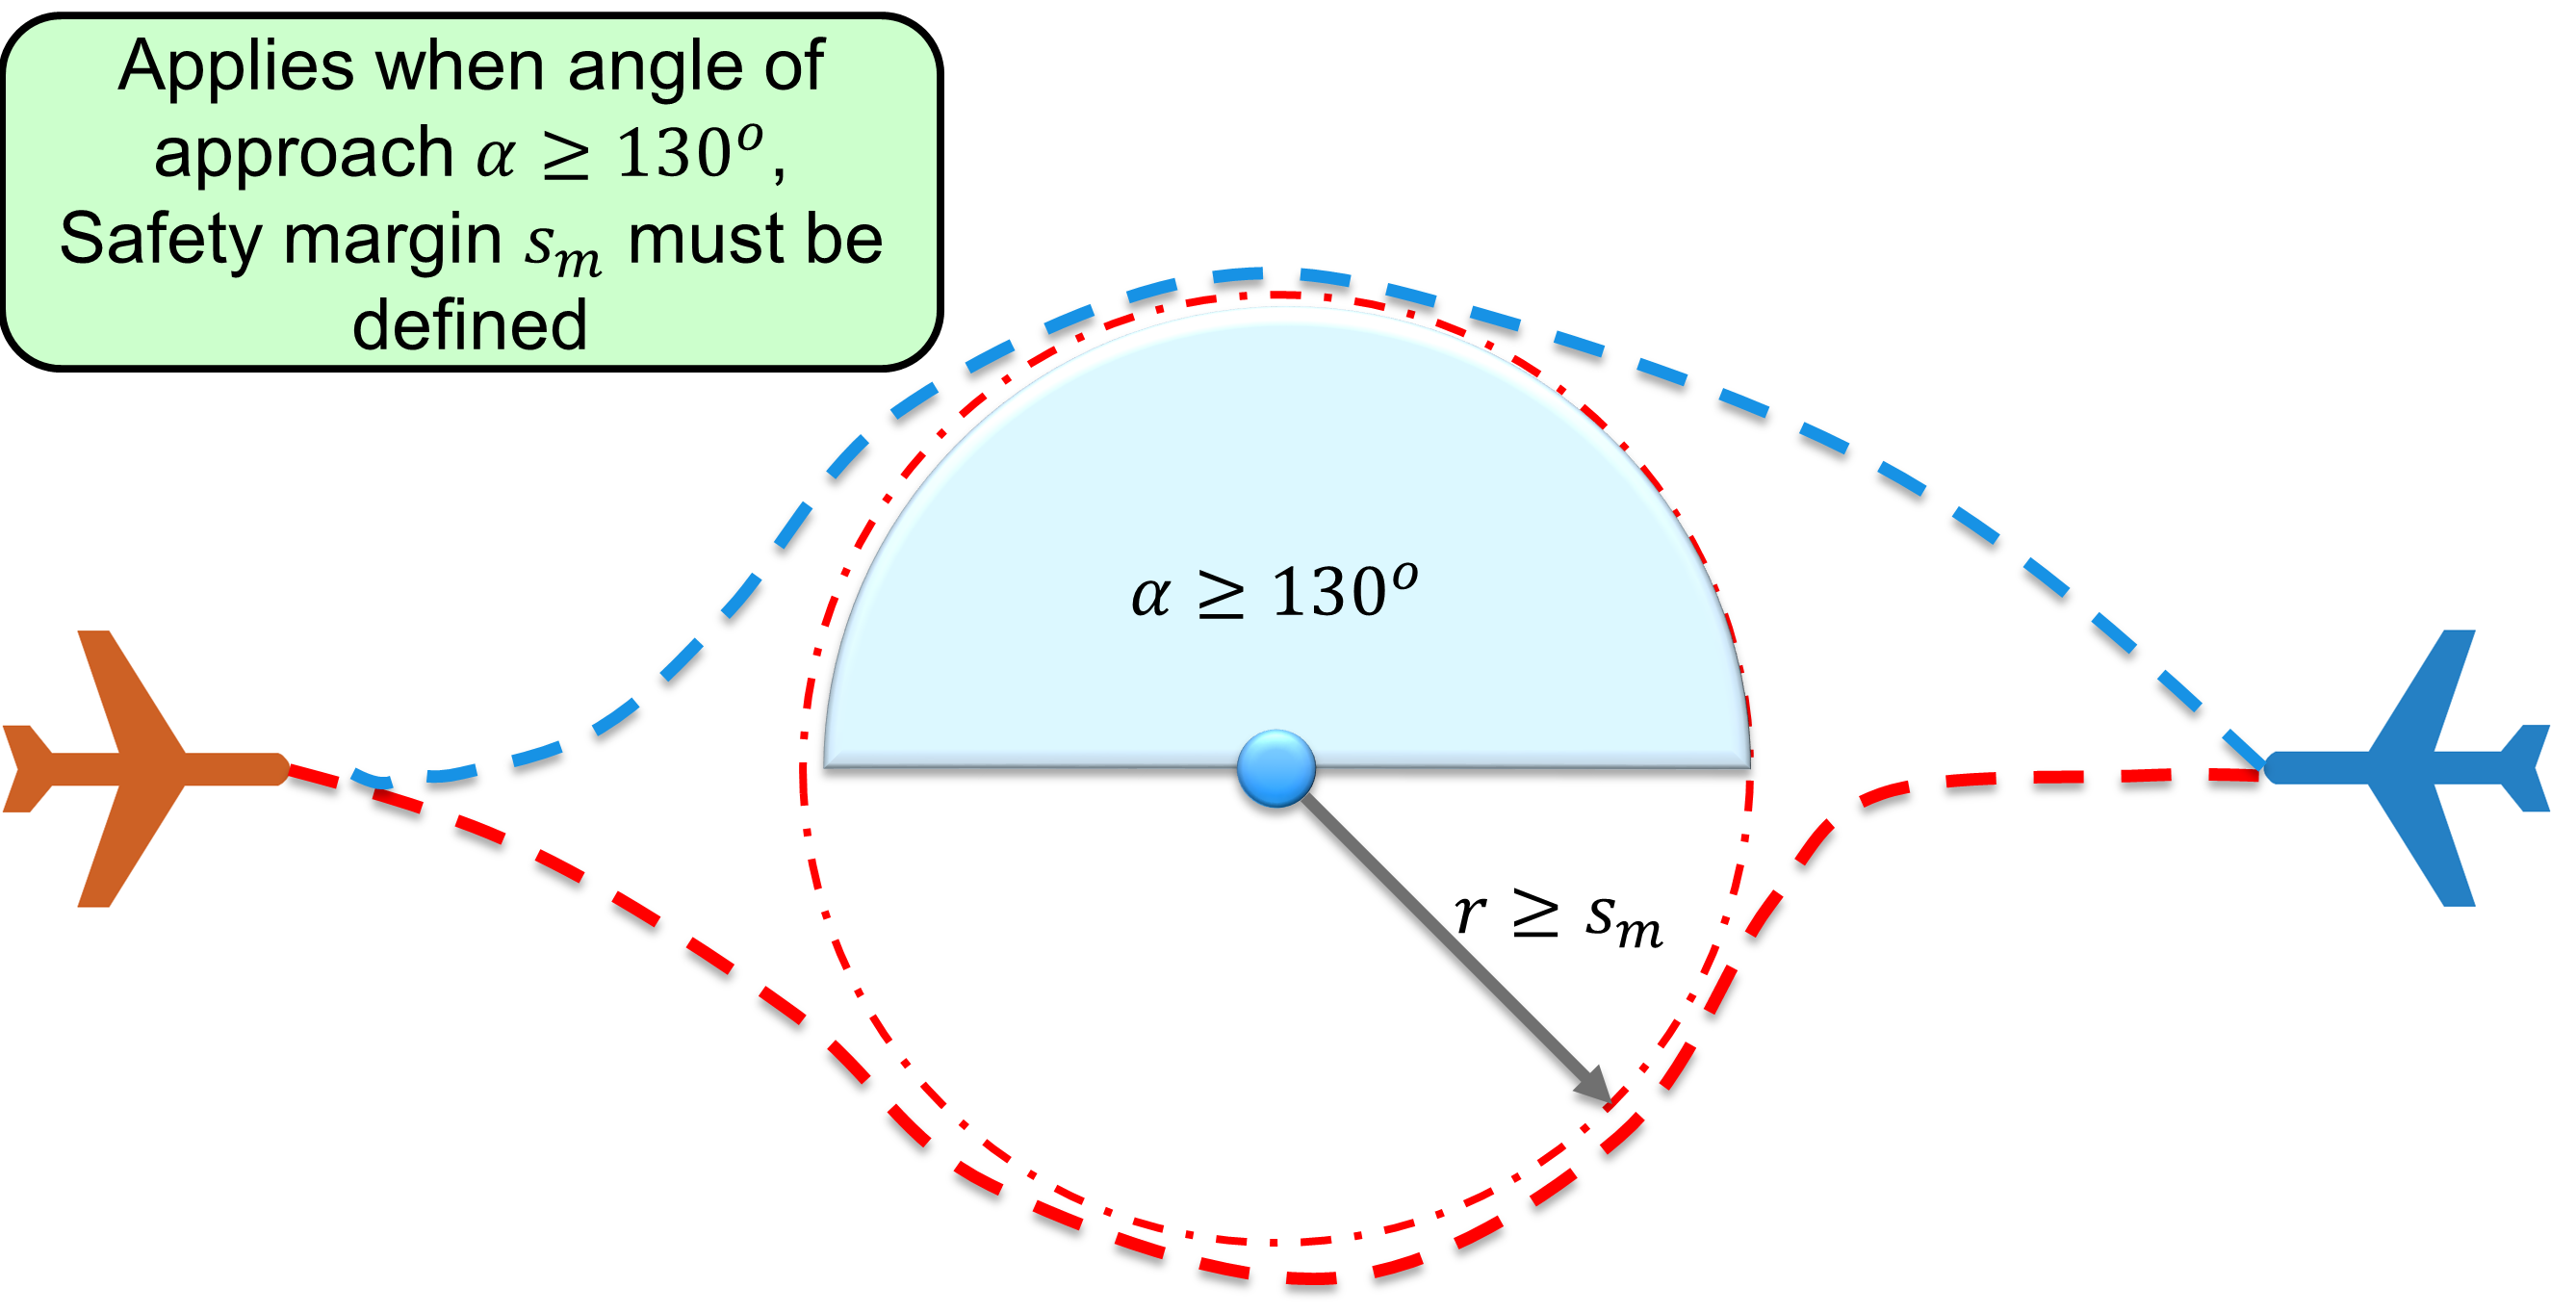
\includegraphics[width=0.9\linewidth,height=95pt,keepaspectratio]{\FIGDIR/RE008HeadOnApproach01} 
            \caption{Detection}
            \label{fig:HeadOnApproachTheoreticalDetection}
        \end{subfigure}
        \begin{subfigure}{0.45\textwidth}
        	\centering
            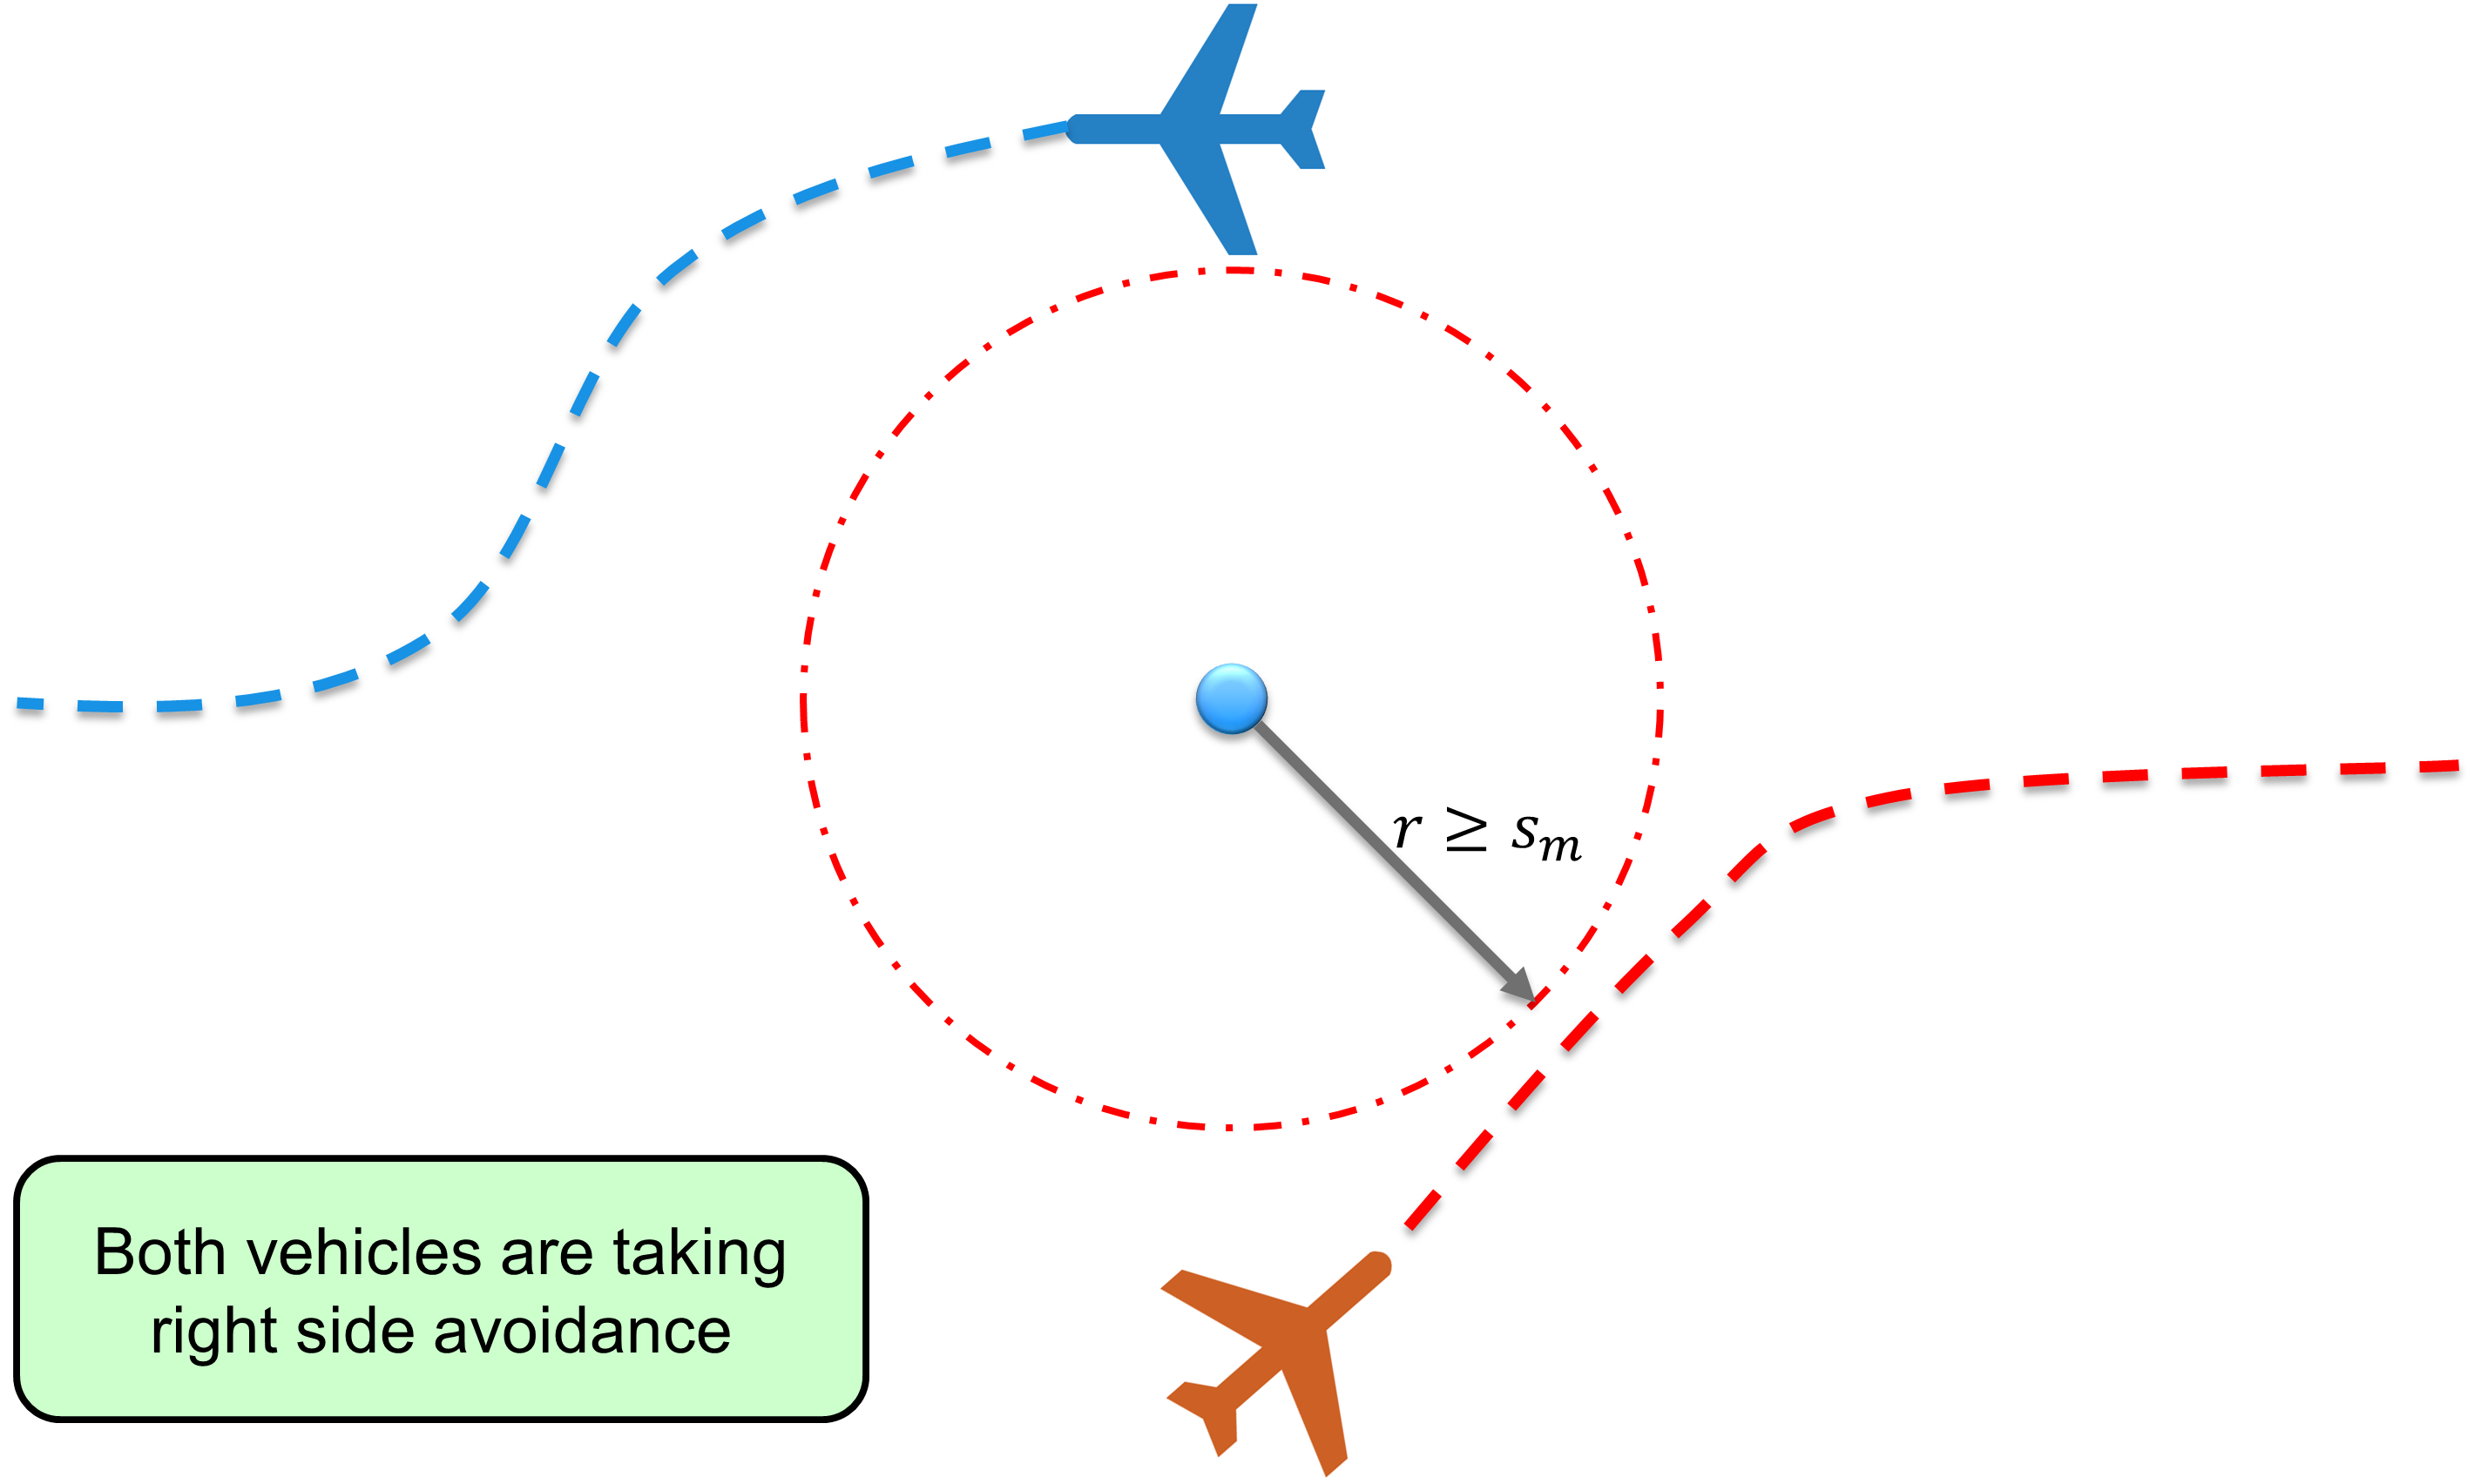
\includegraphics[width=0.9\linewidth,height=95pt,keepaspectratio]{\FIGDIR/RE009HeadOnApproach02} 
            \caption{Resolution/Closure}
            \label{fig:HeadOnApproachTheoreticalResolution}
        \end{subfigure}
        \caption{Head on approach detection/resolution/Closure}
        \label{fig:HeadOnApproachTheoretical}
    \end{figure}
    
\subsection{(W) Handling Converging Maneuver}\label{sec:handlingConvergingManuever}
    \begin{itemize}
        \item Same as Head on approach for most part,
        \item Introduce tilt right concept from highways, emphatize the wake turbulence impact based on angle of approach, 
        \item lesser angle of approach means stronger wake turbulence effect and need to increase or adjust safety margin 
        \item Wake turbulence is represented as dropplet at the back of the plane and can be calculated based on wake turbulence cone from collision case
    \end{itemize}
    \begin{figure}[H]
    	\centering
        \begin{subfigure}{0.32\textwidth}
        	\centering
            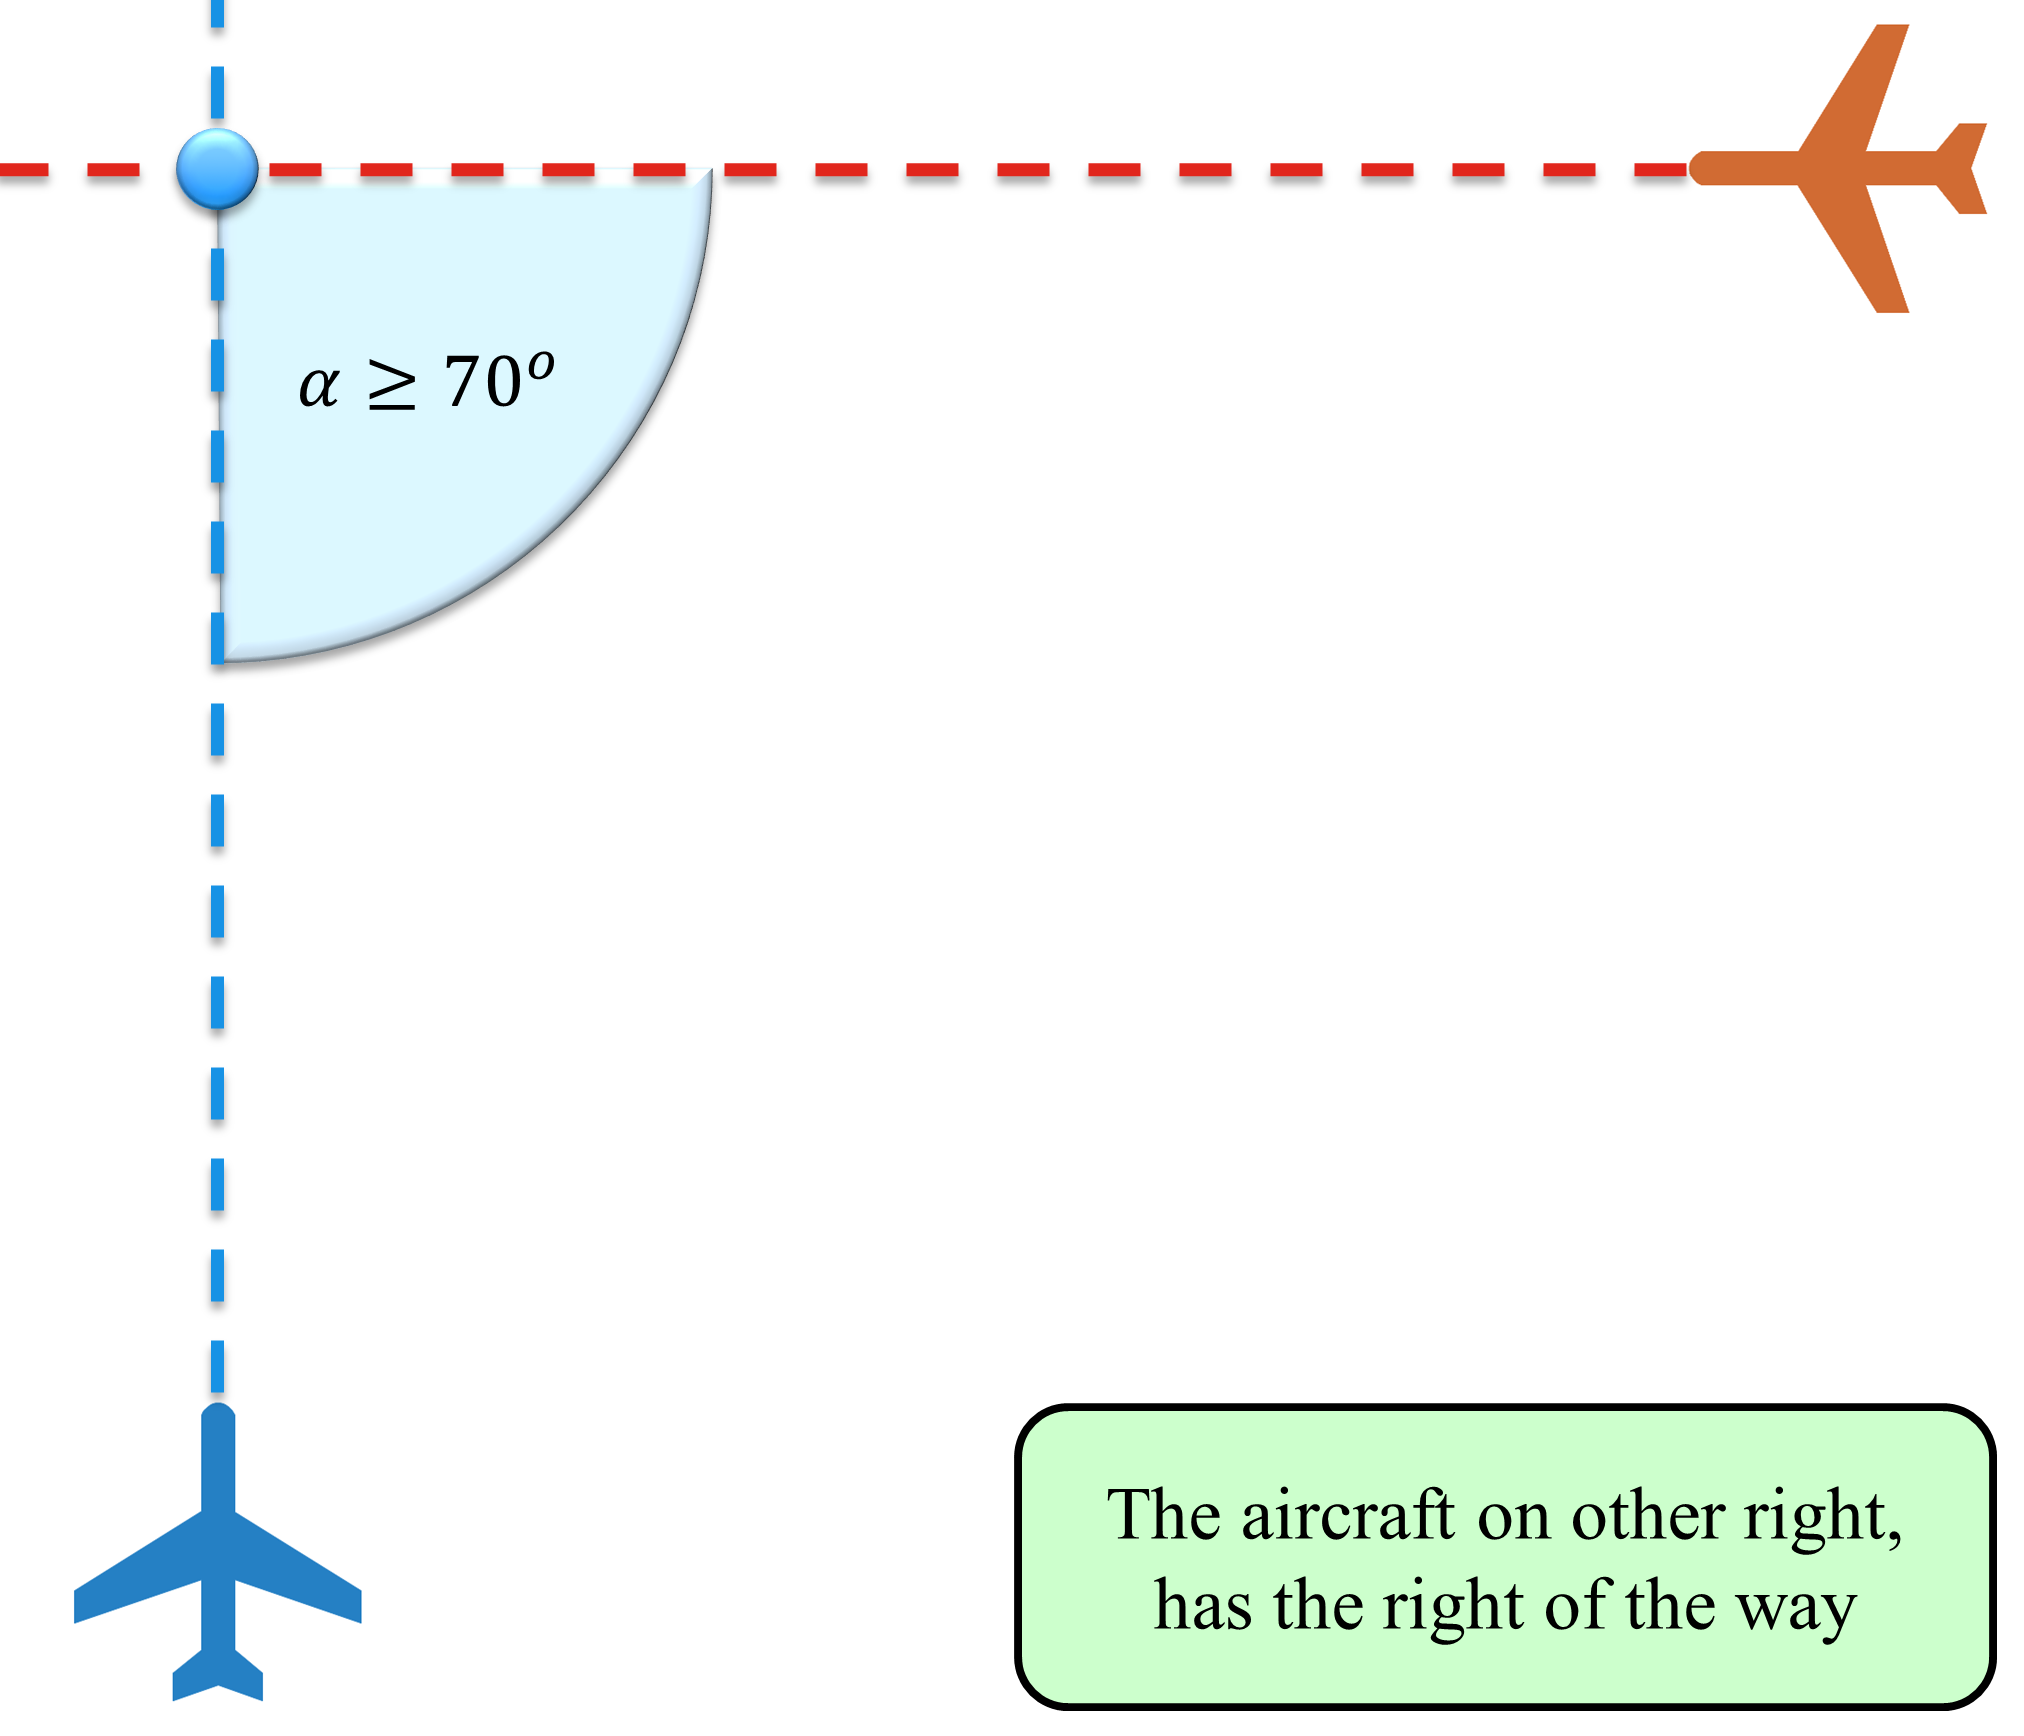
\includegraphics[width=0.9\linewidth,height=105pt,keepaspectratio]{\FIGDIR/RE005ConvergingManeuver01} 
            \caption{Detection}
            \label{fig:ConvergingManeuverTheoreticalDetection}
        \end{subfigure}
        \begin{subfigure}{0.32\textwidth}
	        \centering
            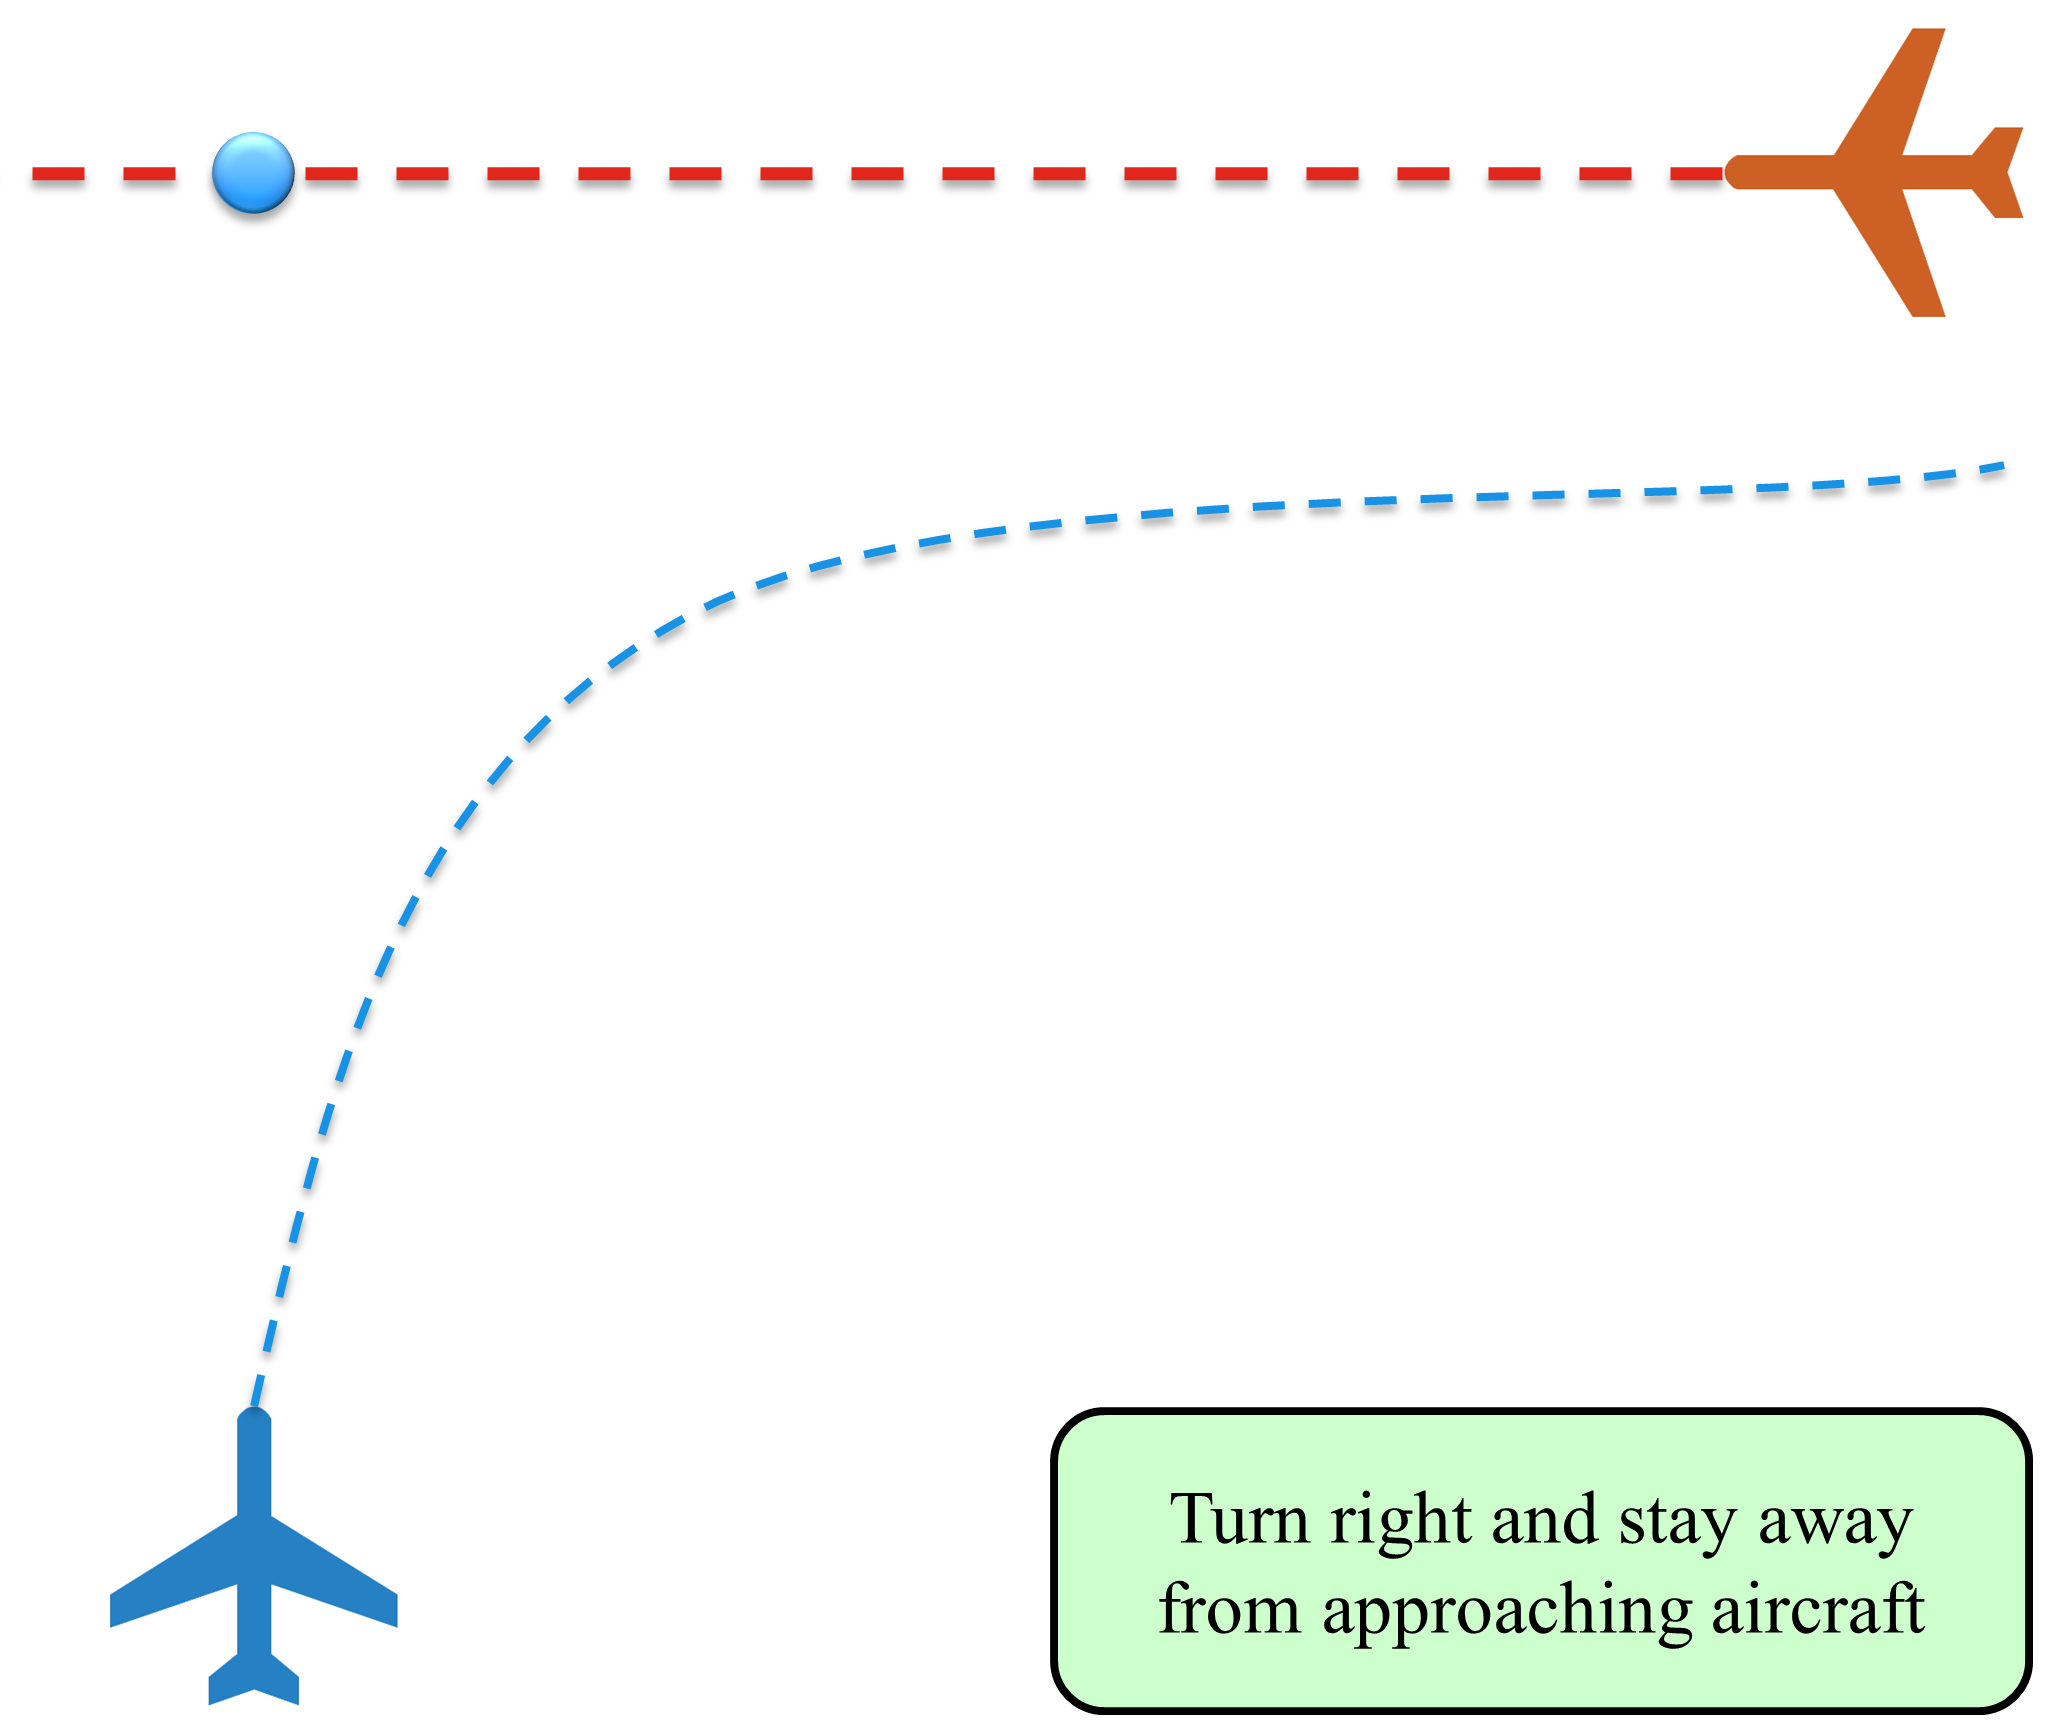
\includegraphics[width=0.9\linewidth,height=105pt,keepaspectratio]{\FIGDIR/RE006ConvergingManuever02} 
            \caption{Resolution}
            \label{fig:ConvergingManeuverTheoreticalResolution}
        \end{subfigure}
        \begin{subfigure}{0.32\textwidth}
	        \centering
            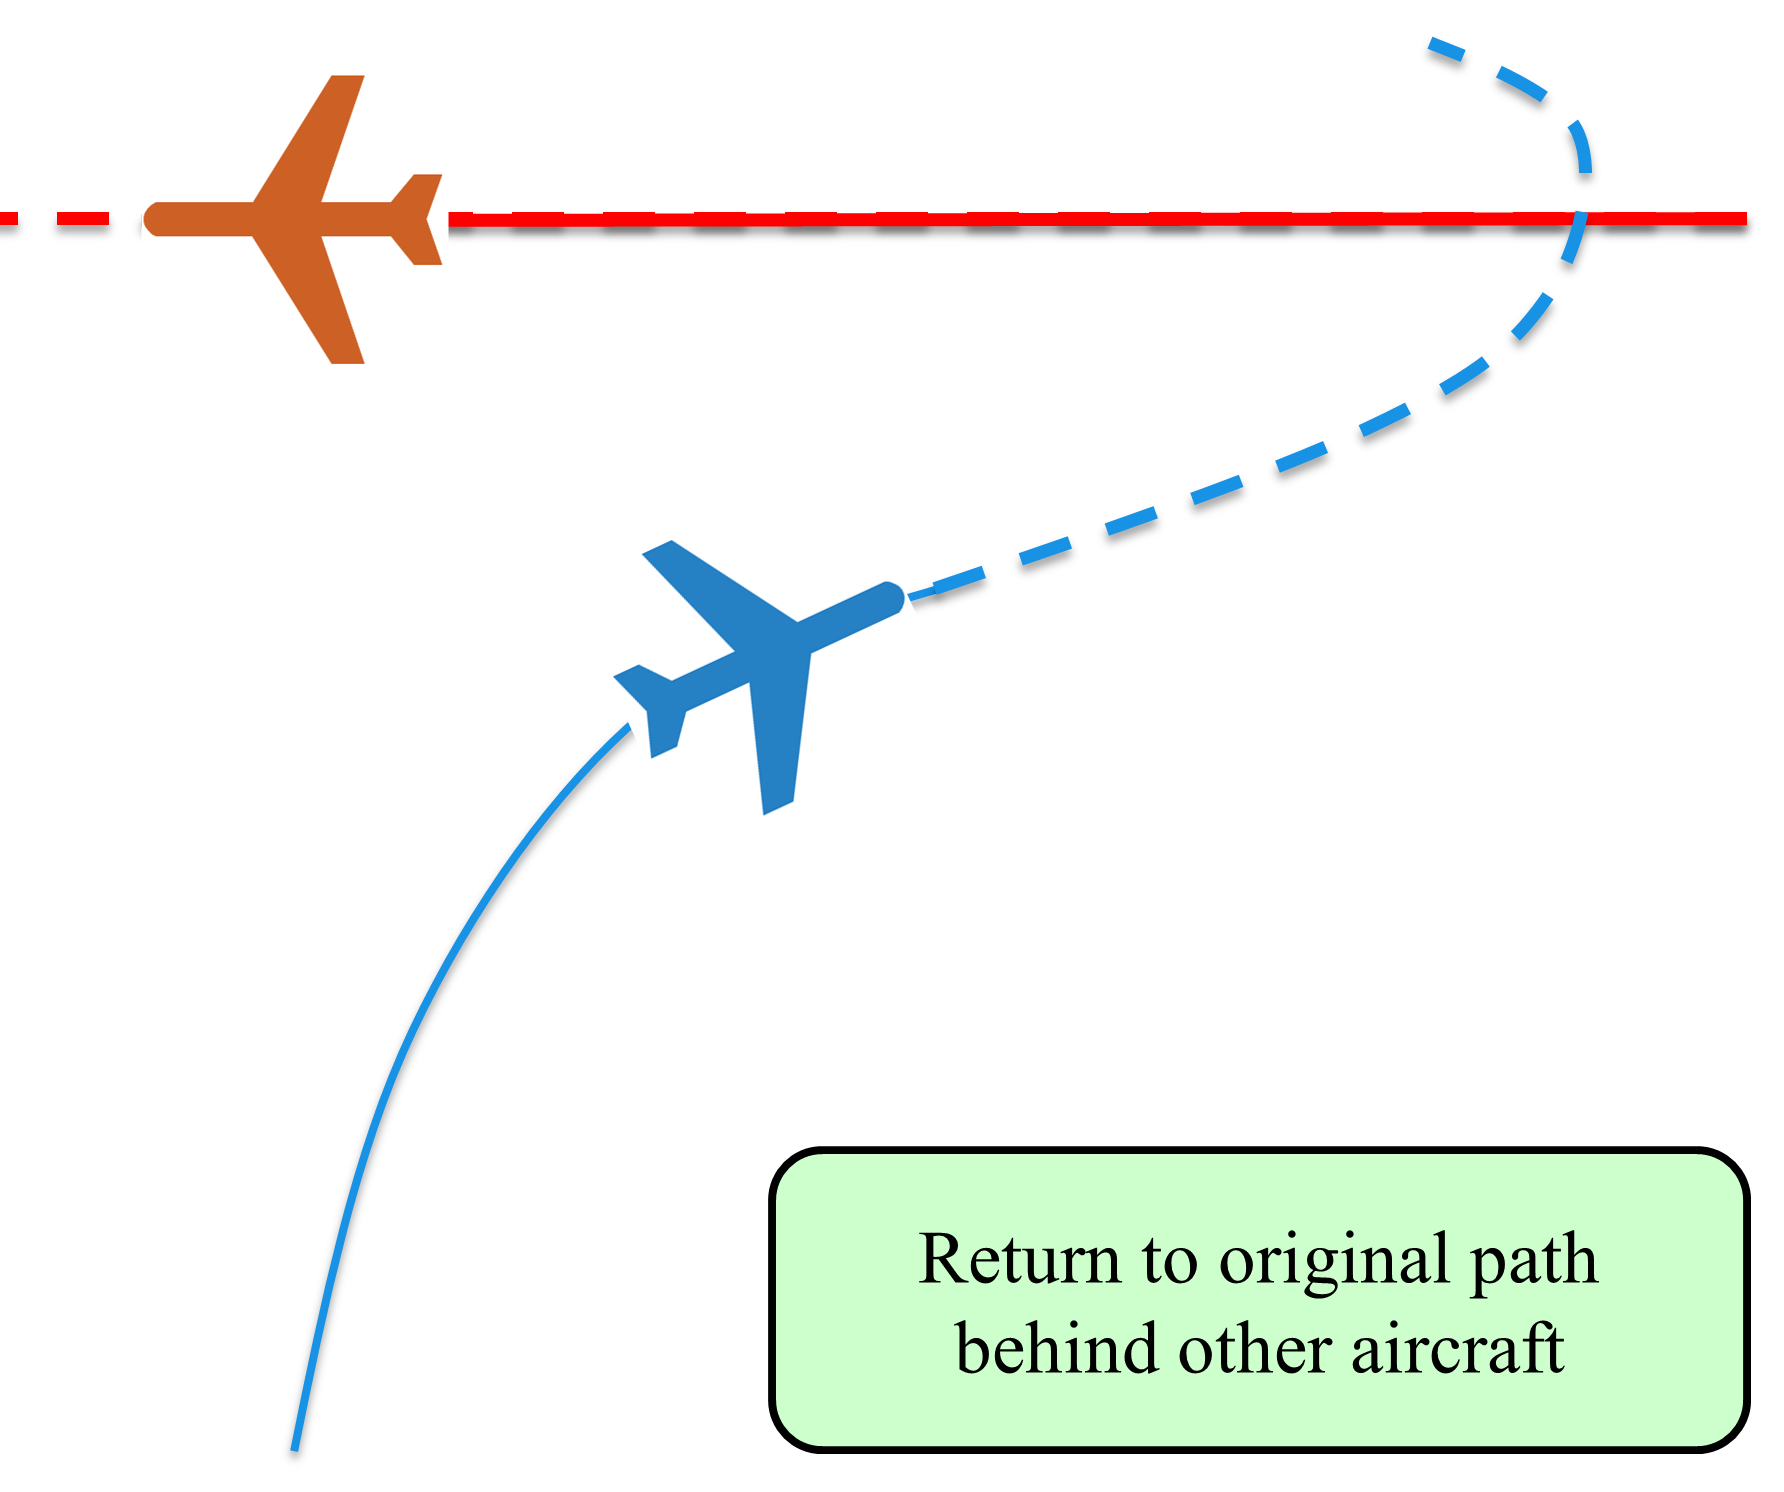
\includegraphics[width=0.9\linewidth,height=105pt,keepaspectratio]{\FIGDIR/RE007ConvergingManuever03} 
            \caption{Closure}
            \label{fig:ConvergingManeuverTheoreticalClosure}
        \end{subfigure}
        \caption{Converging maneuver detection/resolution/Closure}
        \label{fig:ConvergingManeuverTheoretical}
    \end{figure}

\subsection{(W) Handling Overtake Maneuver}\label{sec:handlingOvertakeManuever}
    \begin{itemize}
        \item Emphasize on overtake fragility, there is different speed in controlled airspace,
        \item Fact - most of traffic attendants at same flight level have same cruising speed, de facto lower flight levels are for slower turbo-prop planes and higher altitudes are for jet planes. It is stated that this principle will persist even when UAS will be integrated \cite{bayen2005langrangian,kopardekar2002dynamic,helme1992optimization} via multiple air-traffic models.
        \item Overtake is borderline emergency maneuver, most of conflicts should be solved via virtual round-abounds
    \end{itemize}
    \begin{figure}[H]
    	\centering
        \begin{subfigure}{0.32\textwidth}
            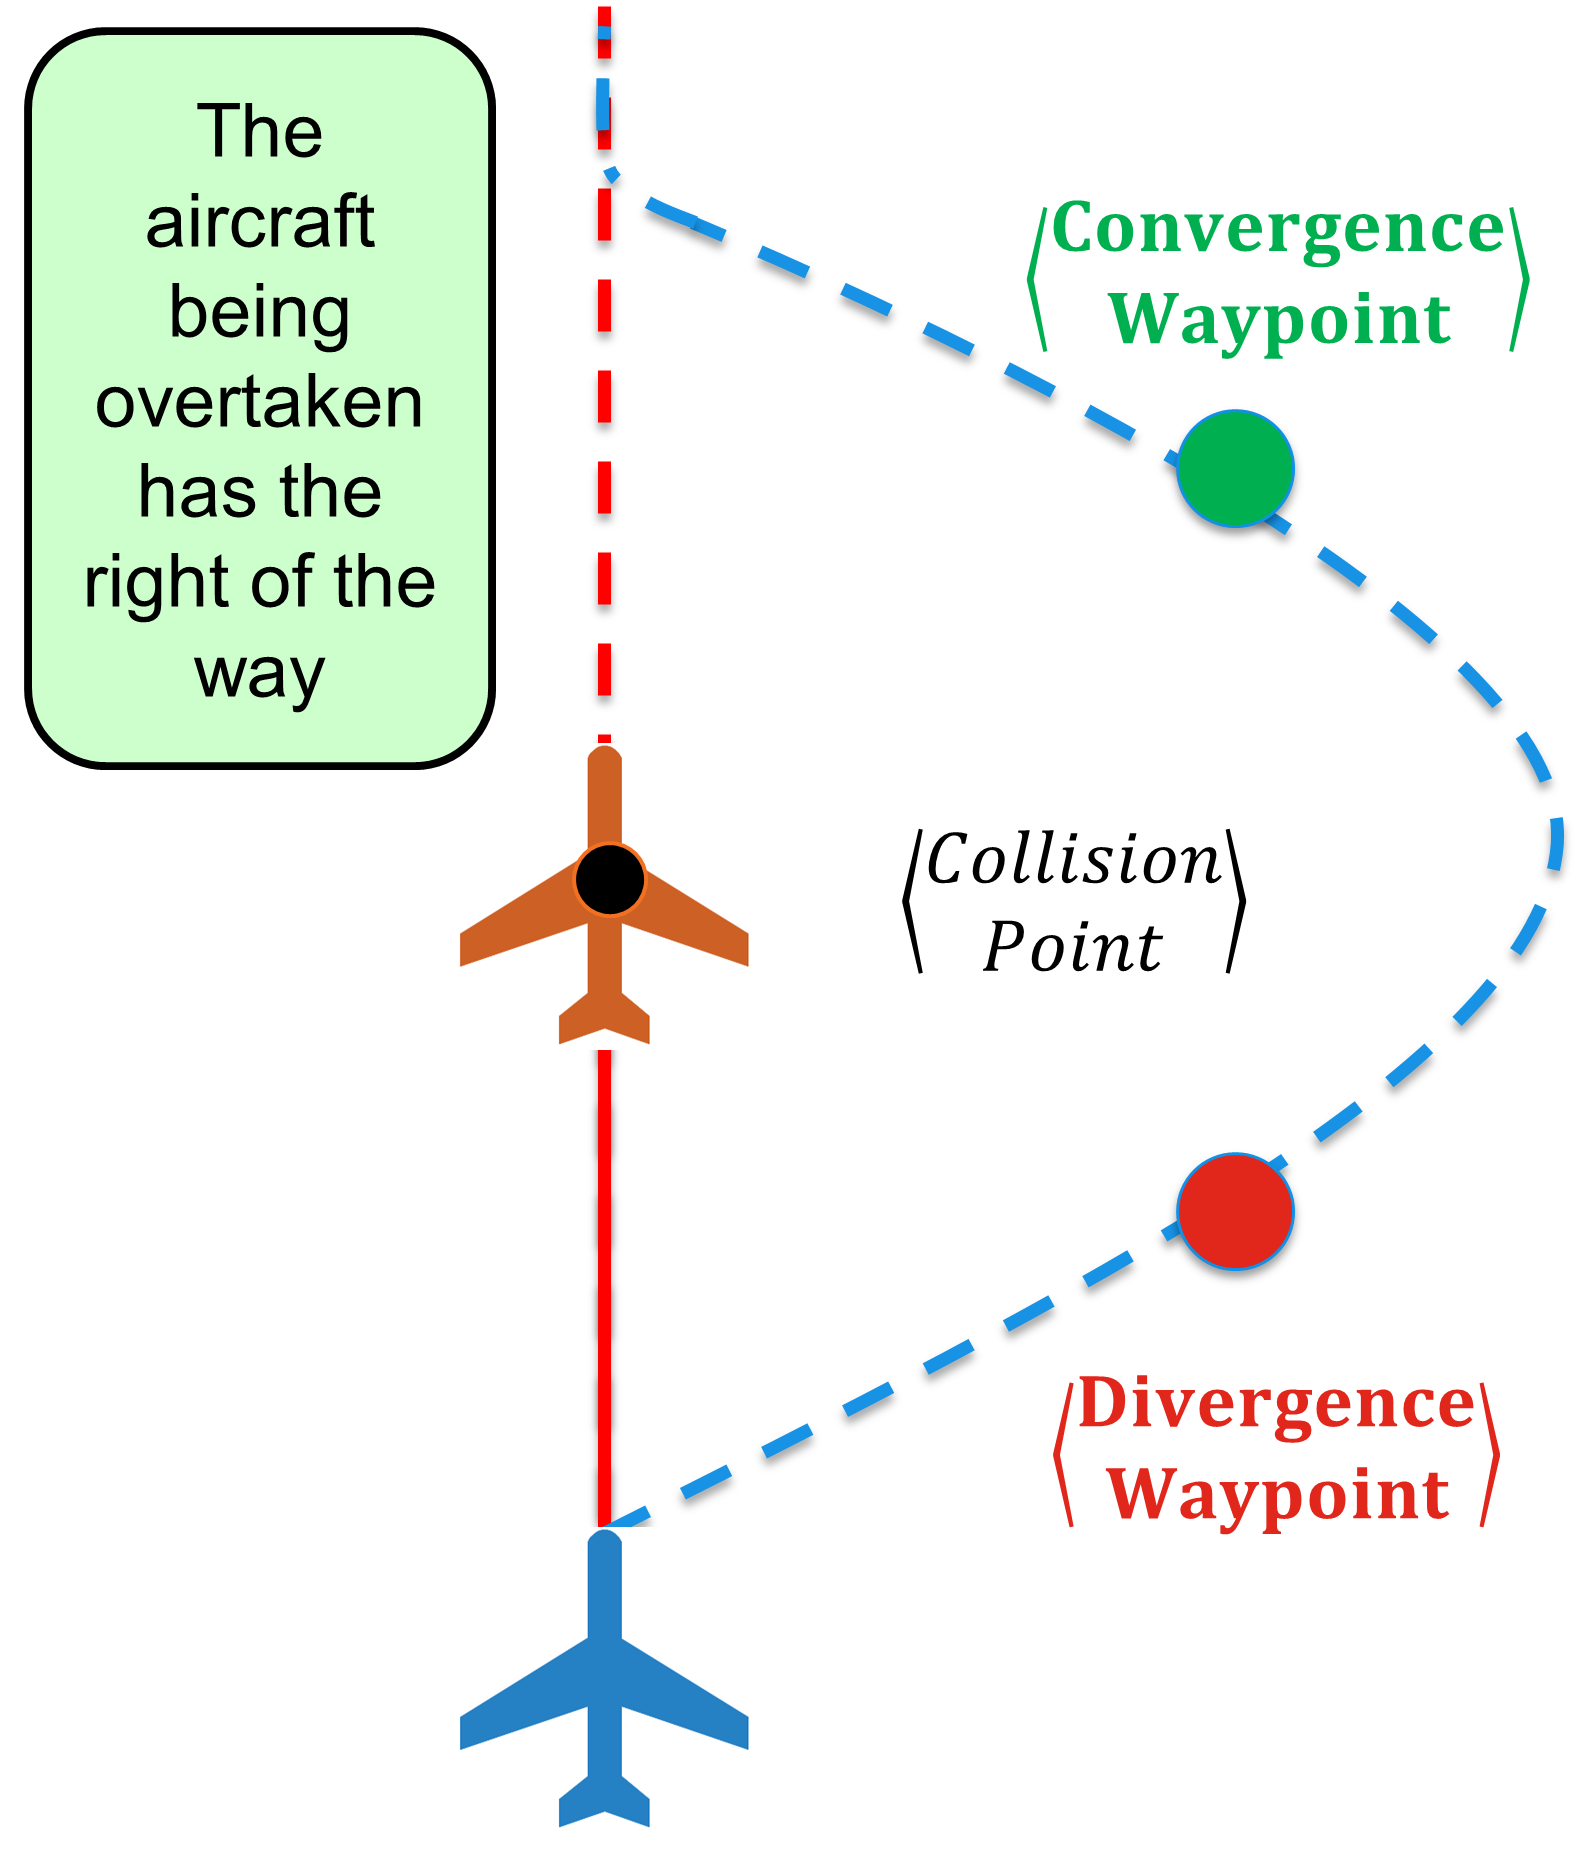
\includegraphics[width=0.9\linewidth,height=142pt,keepaspectratio]{\FIGDIR/RE010OvertakeMAnuever01} 
            \caption{Detection}
            \label{fig:OvertakeManeuverTheoreticalDetection}
        \end{subfigure}
        \begin{subfigure}{0.32\textwidth}
            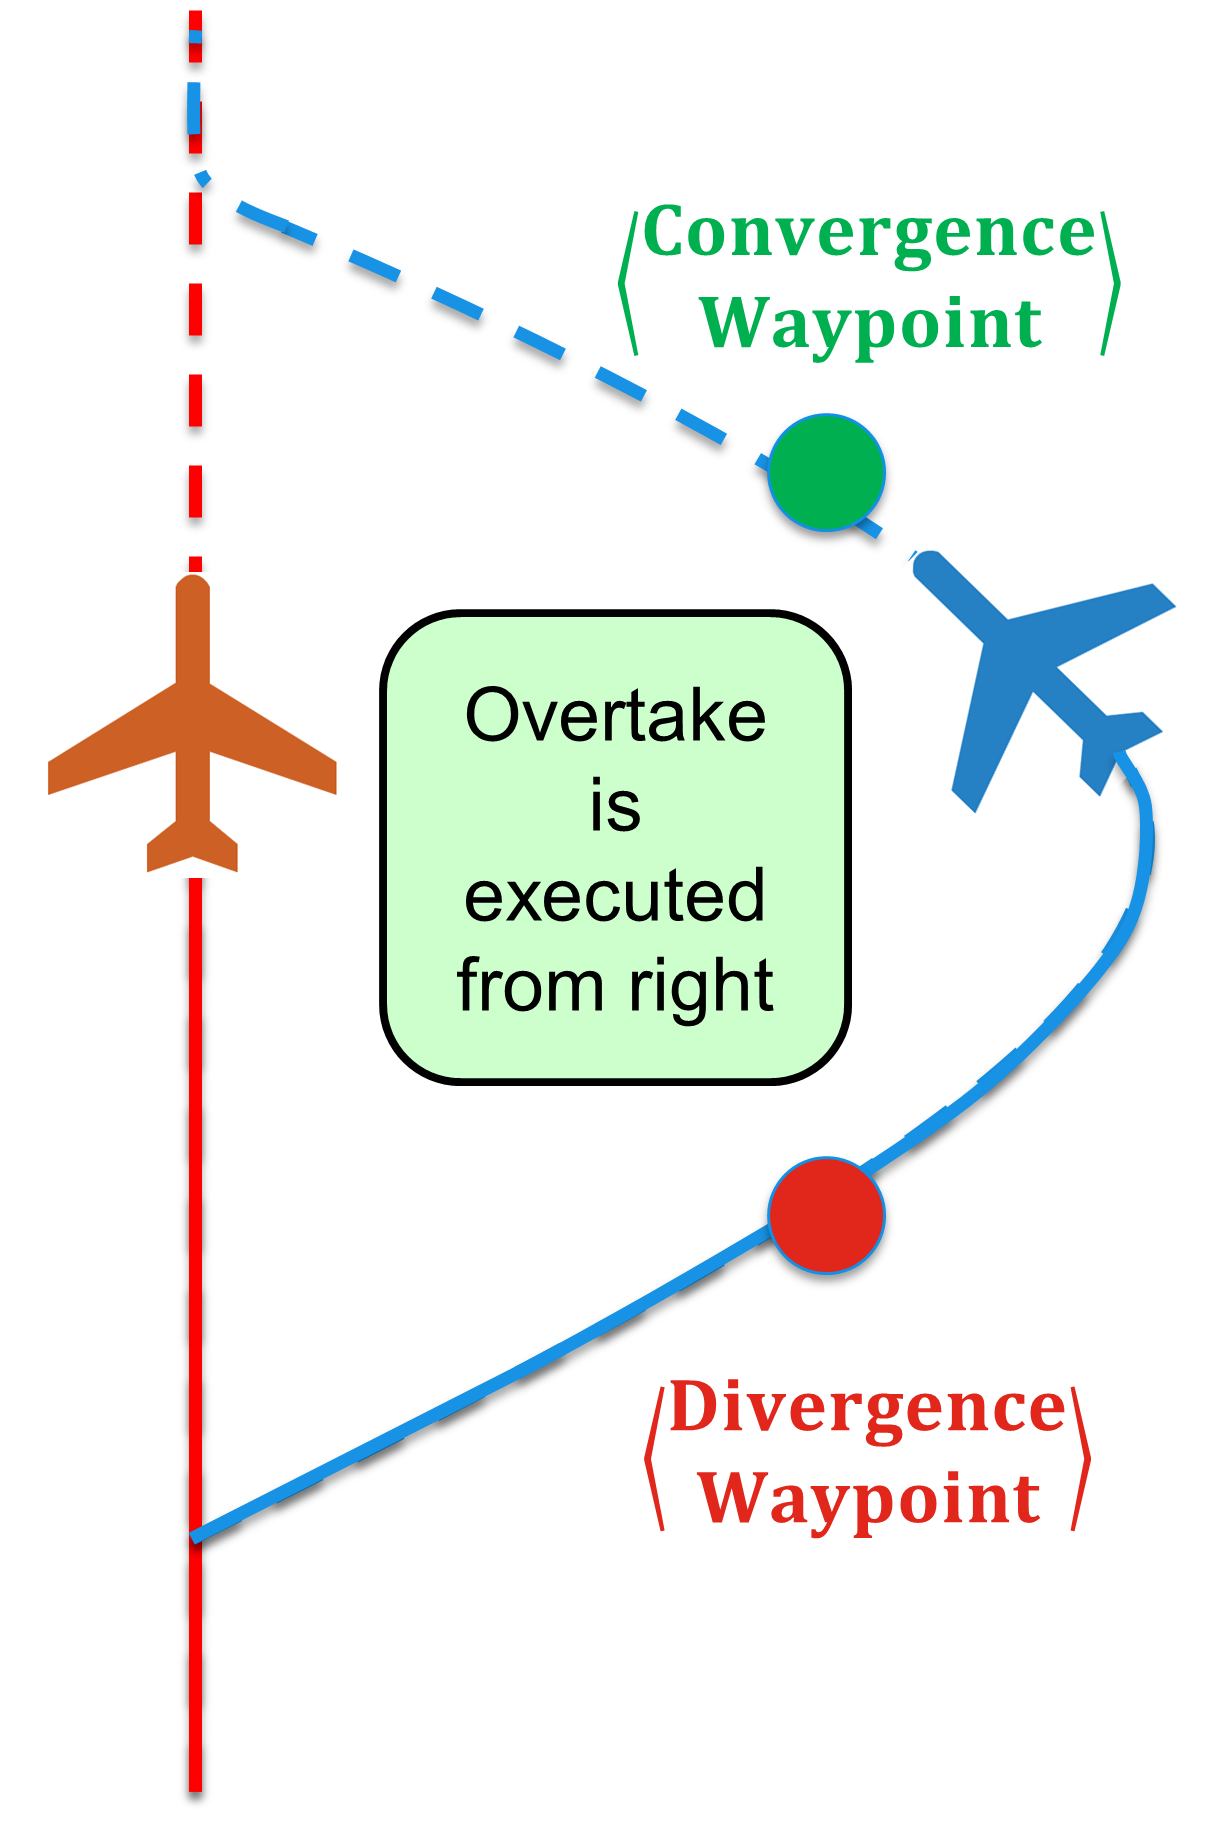
\includegraphics[width=0.9\linewidth,height=142pt,keepaspectratio]{\FIGDIR/RE011OvertakeMAnuever02} 
            \caption{Resolution}
            \label{fig:OvertakeManeuverTheoreticalResolution}
        \end{subfigure}
        \begin{subfigure}{0.32\textwidth}
            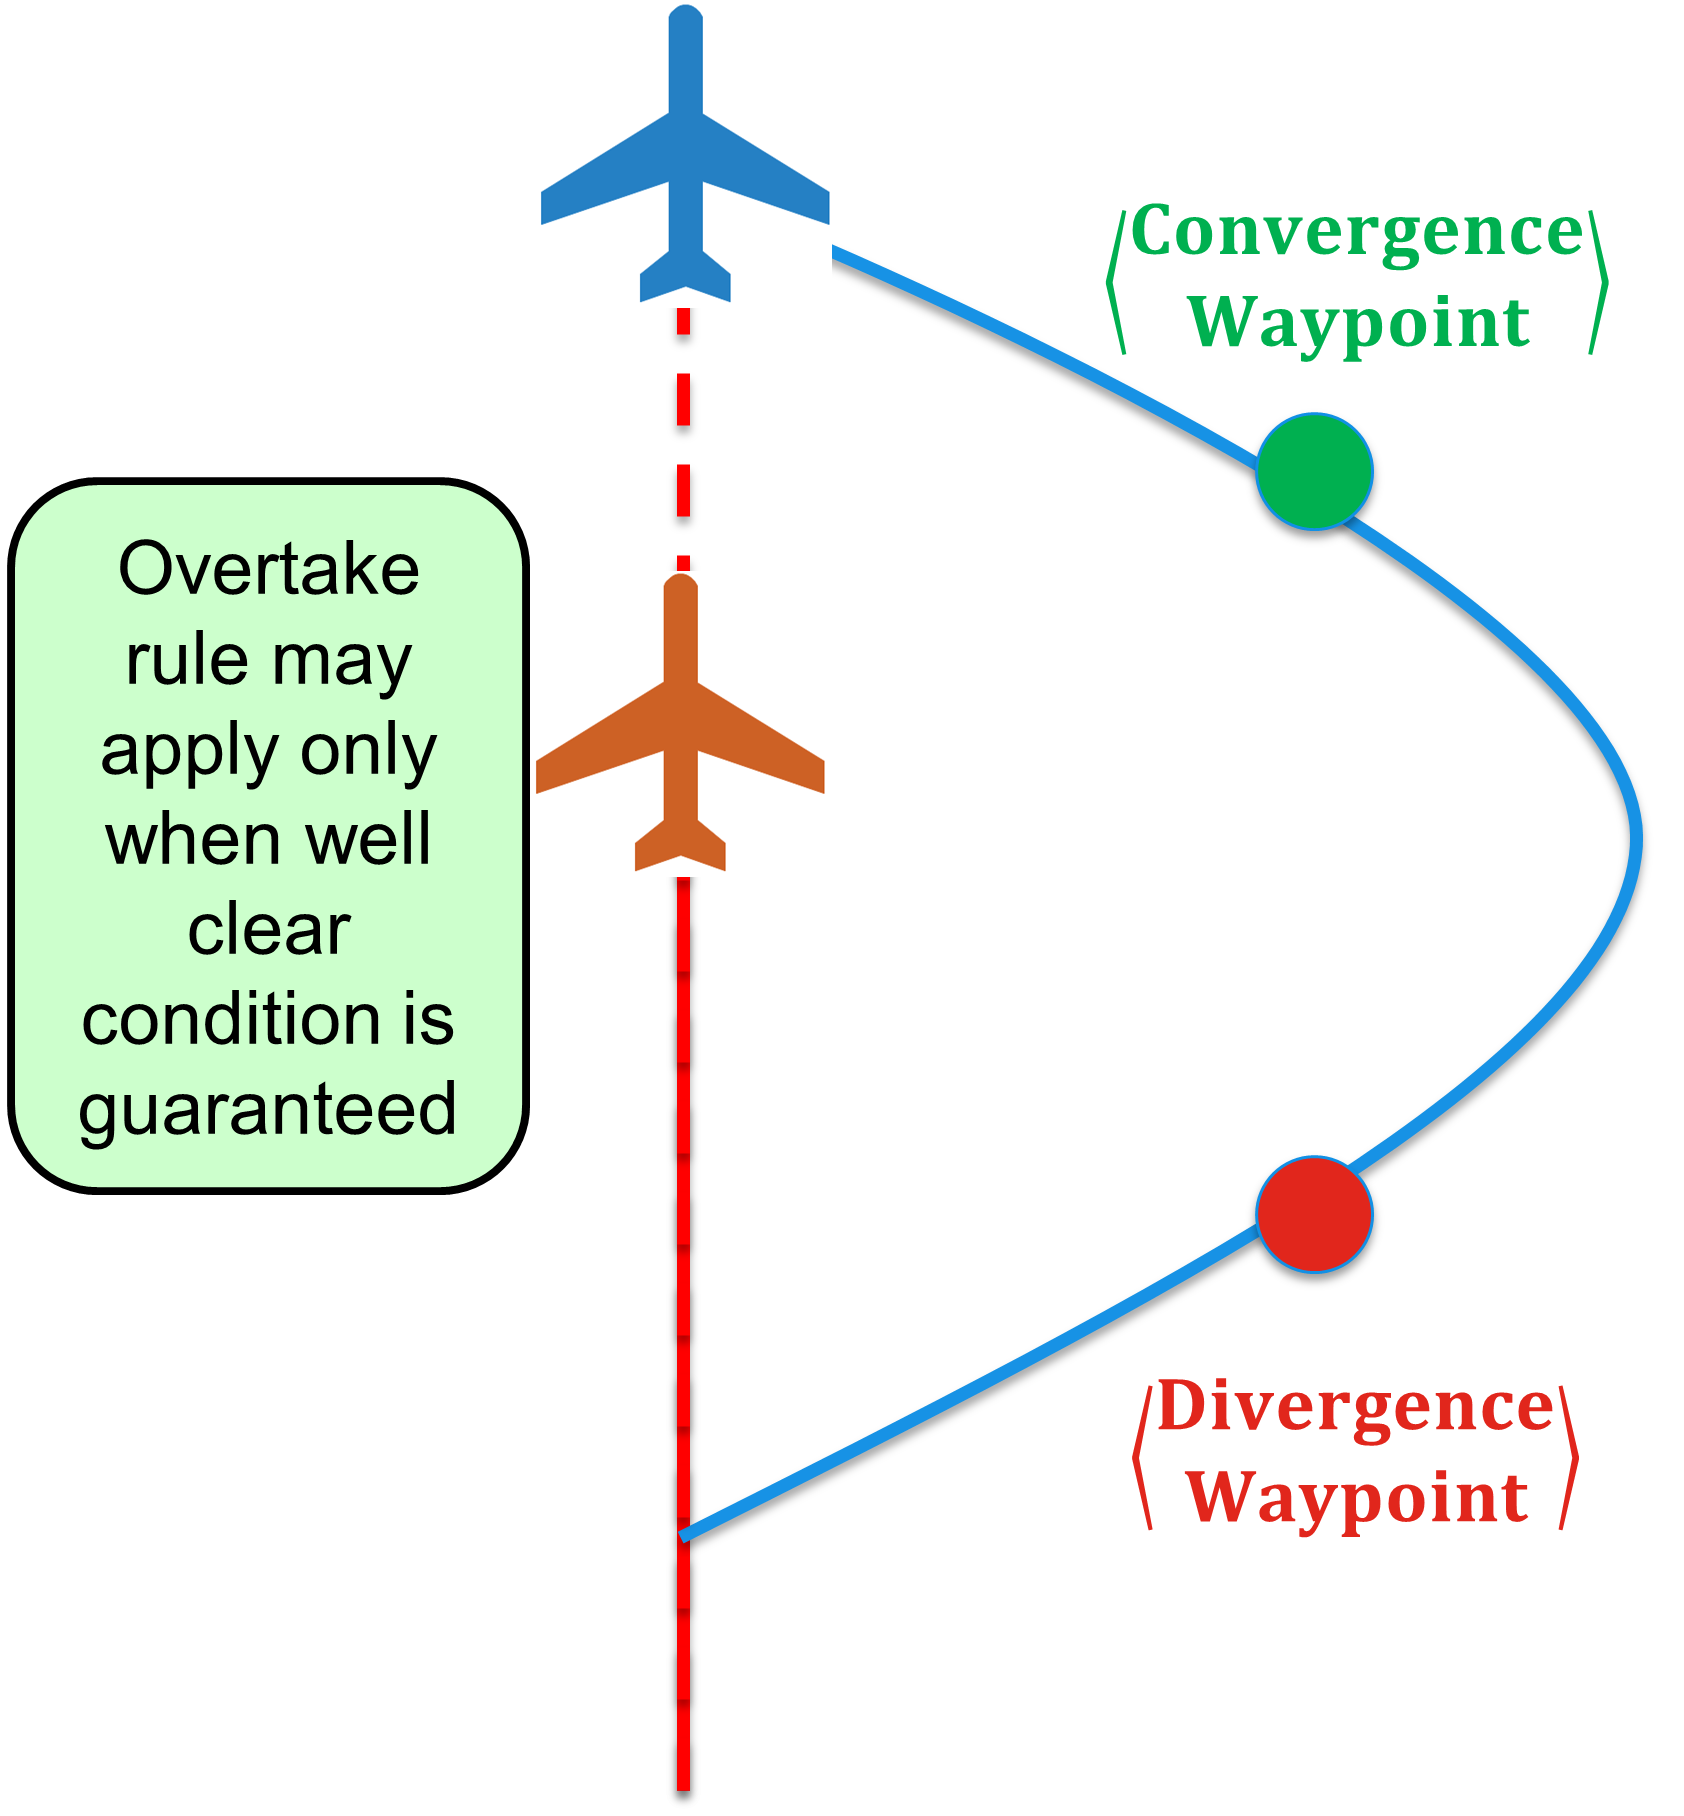
\includegraphics[width=0.9\linewidth,height=142pt,keepaspectratio]{\FIGDIR/RE012OvertakeMAnuever03} 
            \caption{Closure}
            \label{fig:OvertakeManeuverTheoreticalClosure}
        \end{subfigure}
        \caption{Overtake maneuver detection/resolution/Closure}
        \label{fig:OvertakeManeuverTheoretical}
    \end{figure}



